% mallinson-cylinder.tex
%
\newpage
\section{Mallinson's hollow cylinder}
\label{chapter-cylinder}
%
The second validation test case is that of a Mach 8.8 flow 
over a hollow cylinder. This test case is basically an axisymmetric
analogy of the flat plate test case examined in Chapter~\ref{chapter-flat-plate}. 
It serves as an excellent exercise to test the axisymmetric turbulence 
terms in the $k$-$\omega$ model. The large experimental data set of surface 
pressure and heat flux provided in Mallinson et. al. \cite{Mallinson2000} 
and in Boyce \& Hillier \cite{Boyce2000} is compared with predictions from 
Eilmer3 simulations. This exercise also explores the $k$-$\omega$ model's
sensitivity to $y+$ values and maximum cell aspect ratios.

%------------------------------------------------------------------
\subsection{Details of flow problem}
%\label{}
%
The experimental setup used by Mallinson et al. is shown 
schematically in Figure~\ref{figure-cylinder-exp-setup}.
%
\begin{figure}[htbp]
\begin{center}
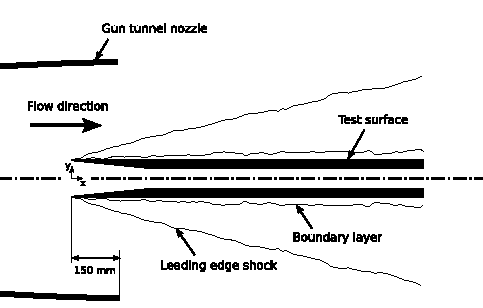
\includegraphics[width=13cm]{./chap3-mallinson-cylinder/figs/experimental-setup.pdf}
\end{center}
\caption{Schematic diagram of the experimental setup for the hollow 
         cylinder test case}
\label{figure-cylinder-exp-setup}
\end{figure}
%
A turbulent boundary layer was allowed to grow on a hollow sharp-nosed 
cylindrical centrebody that had been aligned with a hypersonic flow 
produced by the Imperial College Gun Tunnel. This boundary layer was 
allowed to transition naturally to turbulence from its laminar 
state. Since the test surface was the external surface of the cylinder, 
this test case had the advantage that the body surface was offset from 
the tunnel axis, hence avoiding any centreline focusing effects. The
cylinder was 850\,mm long and had an outer diameter of 75\,mm. The leading
edge of this cylinder was positioned 150\,mm upstream of the nozzle exit
plane for these experiments.

An extensive calibration of the nozzle outflow was conducted by 
Mallinson et. al. to provide as precise a specification of 
freestream flow conditions as possible. Using the static pressure
measured on the surface of the hollow cylinder together with
the reservoir static pressure, freestream pitot pressure 
and stagnation point heat flux, the Mach number was inferred.
The inferred Mach number with axial and radial static pressure 
distributions were then used for a Method-of-Characteristics (MOC) 
calculation to determine the flow conditions at the leading edge
of the hollow cylinder.

The MOC calculations revealed that the nozzle outflow was not exactly 
uniform; the outflow was somewhat radial. The outflow diverged from the
axis of the nozzle by about 0.005$^{\circ}$ per millimetre. As the 
outflow was radial, there was also an axial gradient, $\delta M /\delta x$, 
of about 0.24 per metre. Nominal conditions at the leading edge of the 
cylinder are shown in Table~\ref{inflow-conditions-cylinder}. 
%
\begin{table}[h]
  \caption{Nominal inflow conditions for hollow cylinder test case}
  \label{inflow-conditions-cylinder}
  \begin{center}
    \begin{tabular}{cccl}
      \hline\hline
      Parameter & Value   & Units \\
      \hline
      Test gas    & Nitrogen &    \\
      $M_{\infty,nominal}$  & 8.8      &     \\
      $p_{\infty,nominal}$  & 3.3e3    & Pa  \\
      $T_{\infty,nominal}$  & 69.7     & K   \\
      $u_{\infty,nominal}$  & 1498.0   & m/s \\
      \hline \hline
    \end{tabular}
  \end{center}
\end{table}
%
Static pressure distributions on the cylinder surface were measured 
using Kulite XCS-093 pressure transducers. Wall surface temperature 
time histories measured using platinum/MACOR thin film gauges were 
used together with Schultz \& Jones' theory \cite{Schultz1973} to infer the 
values of surface heat flux. The pressure transducers and thin film 
gauges were located in axial arrays at 120$^{\circ}$ pitch around 
the outside circumference of the hollow model. Uncertainties in the 
static pressure and heat flux measurements were estimated to be 
$\pm$4\% and $\pm$5\% respectively. Experimentally measured values 
of static pressure and heat flux along the cylinder wall are used 
for comparison with results from Eilmer3 simulations. 


%------------------------------------------------------------------
\subsection{Details of computational approach}
%\label{}
%
The setup of the mesh for this test case is similar to that
previously used in the flat plate test case in Chapter~\ref{chapter-flat-plate}.
While the test case in Chapter~\ref{chapter-flat-plate} was aimed at
showing the $k$-$\omega$ model's sensitivity to freestream turbulence
properties, this test case aims to investigate the $k$-$\omega$ model's 
sensitivity to differing grids. Two main aspects of grid configurations
are examined in this chapter - $y^+$ and cell aspect ratio.
\begin{figure}[h]
\begin{center}
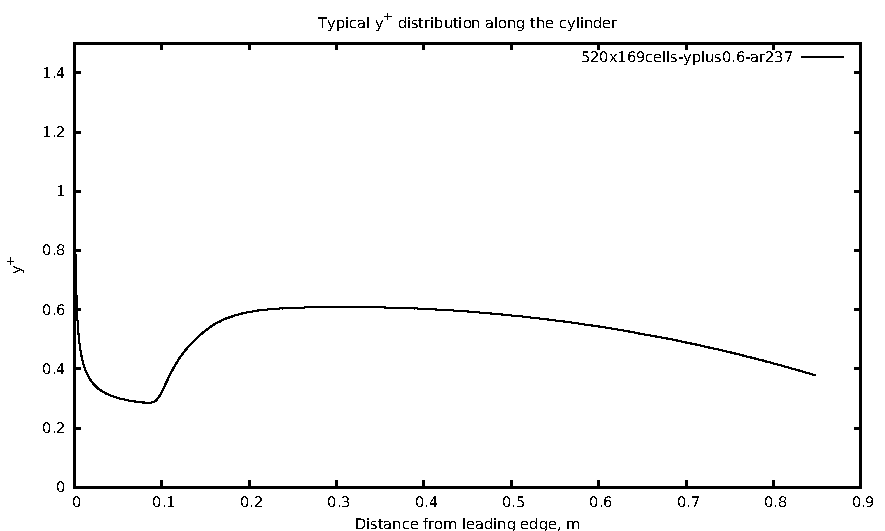
\includegraphics[width=15cm]{./chap3-mallinson-cylinder/figs/typical-yplus-distribution.pdf}
\end{center}
\caption{Typical $y^+$ distribution along the test surface}
\label{figure-cylinder-typical-yplus-dist}
\end{figure}
%
\begin{table}[h]
  \caption{Different grids used for the hollow cylinder test case}
  \label{table-cylinder-grids}
  \begin{center}
    \begin{tabular}{cccccl}
      \hline\hline
      Grid & Number       & Number       & $y^+$ & Maximum \\
           & of $x$-cells & of $y$-cells &       & aspect ratio \\
      \hline
      100x33cells-yplus3.0-ar215   & 100  &  33 & 3.0 & 215 \\
      200x65cells-yplus1.5-ar227   & 200  &  65 & 1.5 & 227 \\
      200x65cells-yplus0.4-ar922   & 200  &  65 & 0.4 & 922 \\
      400x130cells-yplus0.8-ar235  & 400  & 130 & 0.8 & 235 \\
      400x130cells-yplus1.7-ar114  & 400  & 130 & 1.7 &  92 \\
      400x130cells-yplus0.2-ar961  & 400  & 130 & 0.2 & 961 \\
      400x130cells-yplus0.2-ar864  & 400  & 130 & 0.2 & 864 \\
      600x130cells-yplus0.2-ar577  & 600  & 130 & 0.2 & 577 \\
      520x169cells-yplus0.6-ar237  & 520  & 169 & 0.6 & 237 \\
      \hline \hline
    \end{tabular}
  \end{center}
\end{table}
%
\begin{figure}[h]
 \begin{center}
  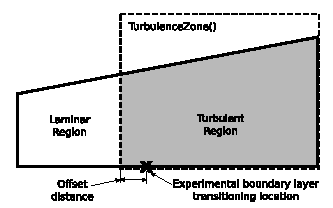
\includegraphics[width=10cm]{./chap3-mallinson-cylinder/figs/turbulence-zone.pdf}
 \end{center}
 \caption{Offset distance to estimate the start of the \texttt{TurbulenceZone()}}
 \label{figure-cylinder-turbulence-zone}
\end{figure}


Table~\ref{table-cylinder-grids} shows the different grids that were used.
Note that the $y^+$ specified in the fourth column of Table~\ref{table-cylinder-grids}
is only an averaged $y^+$ value taken between $x$ = 0.2\,m and $x$ = 0.8\,m
- a typical $y^+$ distribution along the test surface is shown in 
Figure~\ref{figure-cylinder-typical-yplus-dist}.

The test gas used was nitrogen with an ideal gas assumption, a 
constant specific heats ratio of 1.4 and a gas constant of 296.8\,J/kg.K. 
An isothermal wall at a temperature of 295\,K was used. 
The setup of the supersonic inflow boundary condition is different
to the flat plate test case due to the presence of flow angularity
in the inflow. This angularity was taken into account by using the 
user-defined boundary condition \texttt{UserDefinedBC("")} 
available in Eilmer3. An example showing the usage of \texttt{UserDefinedBC("")}
can be found in the Eilmer3 user guide. For this test case,
this boundary condition was specified by adding  \texttt{UserDefinedBC("udf-supersonic-in.lua")} 
in the \textit{Python} setup script. The \texttt{udf-supersonic-in.lua} file 
is shown in Section~\ref{section-udf-supersonic-in-lua}.

The $k$-$\omega$ model has always been known to predict premature
transitioning for boundary layers \cite{Wilcox2006}. To counteract this 
and simulate boundary layer transitioning, an initial simulation was
performed to estimate the transition location predicted by the 
$k$-$\omega$ model. This distance is then used as an offset distance 
to define the start of the turbulent block, as shown in 
Figure~\ref{figure-cylinder-turbulence-zone}.

% Might configure Eilmer3 to use Dan's in-code "heat flux extractor"..
%While surface static pressure can be directly extracted from the 
%simulations, surface heat flux has to be inferred using the 
%temperatures in the first cells along the wall. The heat flux can
%then be computed by ..... blah blah ..

%------------------------------------------------------------------
%\subsection{Grid convergence}
%\label{}
%

%------------------------------------------------------------------
\subsection{Results \& discussion}
%\label{}
%
Figures~\ref{cylinder-bl-profiles}, \ref{cylinder-surface-static-pressure-compare-grid} 
and \ref{cylinder-surface-heat-flux-compare-grid} show the numerical results for 
four different grid resolutions. In contrast to the boundary layer profiles shown 
in Figure~\ref{cylinder-bl-profiles}, the simulated wall static pressure and heat 
flux distribution in Figures~\ref{cylinder-surface-static-pressure-compare-grid} and 
\ref{cylinder-surface-heat-flux-compare-grid} 
do not appear to show any form of grid convergence. Since the wall static pressure 
and heat flux distribution are values taken from the first cells off the wall, this 
indicates that the overall influence on the external flowfield from the wall cells is 
not too significant. If grid convergence was considered based only on the boundary 
layer profiles, the fine grid would have been considered to produce sufficiently 
grid-converged results.
%
\begin{figure}[h]
 \begin{center}
  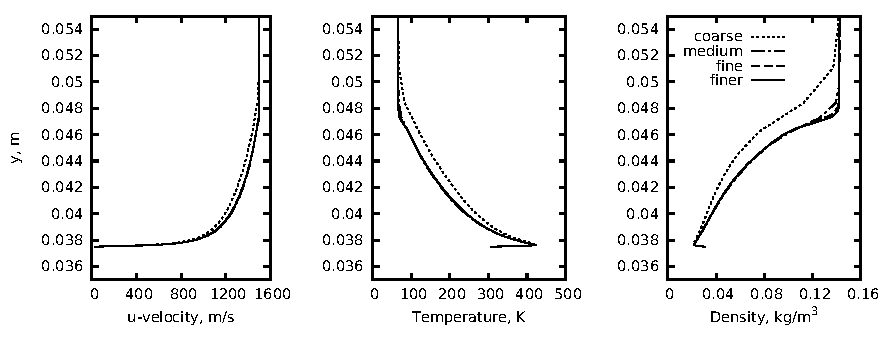
\includegraphics[width=15cm]{./chap3-mallinson-cylinder/figs/boundary-layer-profile-800mm.pdf}
 \end{center}
 \caption{Near wall boundary layer profiles at $x$ = 0.8\,m 
          (where ``coarse" is the ``100x33cells-yplus3.0-ar215" grid, 
          ``medium" is the ``200x65cells-yplus1.5-ar227" grid,
          ``fine" is the ``400x130cells-yplus0.8-ar235" grid, and
          ``finer" is the ``520x169cells-yplus0.6-ar237" grid.)}
 \label{cylinder-bl-profiles}
\end{figure}
\begin{figure}[h]
 \begin{center}
  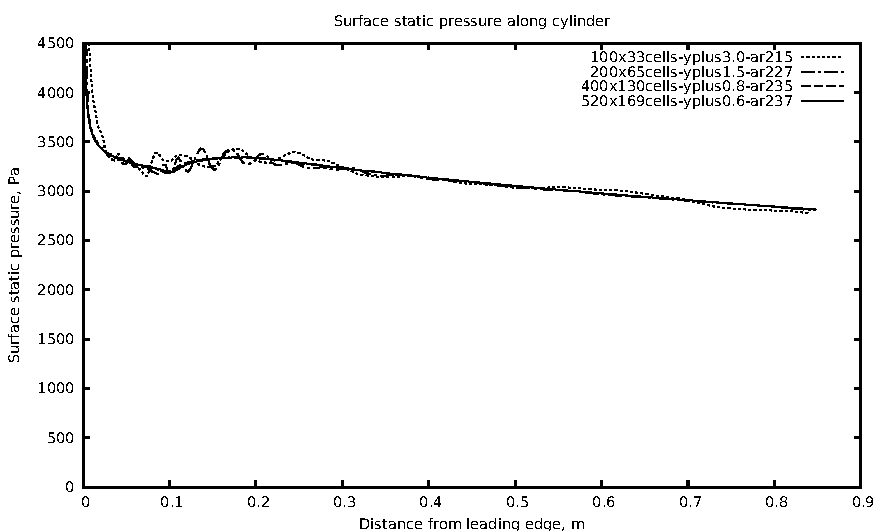
\includegraphics[width=15cm]{./chap3-mallinson-cylinder/figs/compare-grid-resolution-pressure.pdf}
 \end{center}
 \caption{Surface static pressure distribution for different grid resolutions}
 \label{cylinder-surface-static-pressure-compare-grid}
%\end{figure}
%\begin{figure}[h]
\vspace{2cm}
 \begin{center}
  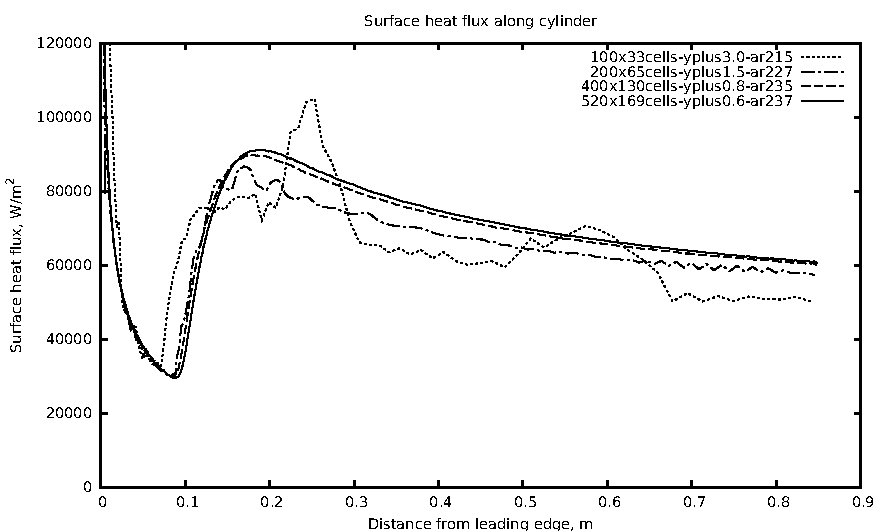
\includegraphics[width=15cm]{./chap3-mallinson-cylinder/figs/compare-grid-resolution-heat-flux.pdf}
 \end{center}
 \caption{Surface heat flux distribution for different grid resolutions}
 \label{cylinder-surface-heat-flux-compare-grid}
\end{figure}

The fluctuations in the static pressure and heat flux, and the non-converging heat 
flux values evident in Figures~\ref{cylinder-surface-static-pressure-compare-grid} and 
\ref{cylinder-surface-heat-flux-compare-grid} are likely to be due to the differences in 
the $y^+$ values for each grid. As the grid is refined, the $y^+$ value decreases.
Figures~\ref{cylinder-surface-static-pressure-compare-grid} and \ref{cylinder-surface-heat-flux-compare-grid} 
show that the fluctuations in the wall static pressure and heat flux values are not present for 
grids with $y^+$ values lesser than 1.0 - the minimum $y^+$ value recommended earlier 
in Chapter~\ref{chapter-flat-plate}. To closer examine the influence of $y^+$ on the 
simulations, the grid clustering for the ``400x130cells-yplus0.8-ar235" grid is 
adjusted to vary the $y^+$ values. The simulated wall static pressure and heat flux 
distributions are shown in Figures~\ref{cylinder-surface-static-pressure-compare-yplus}
and \ref{cylinder-surface-heat-flux-compare-yplus} respectively.
%
\begin{figure}[h]
 \begin{center}
  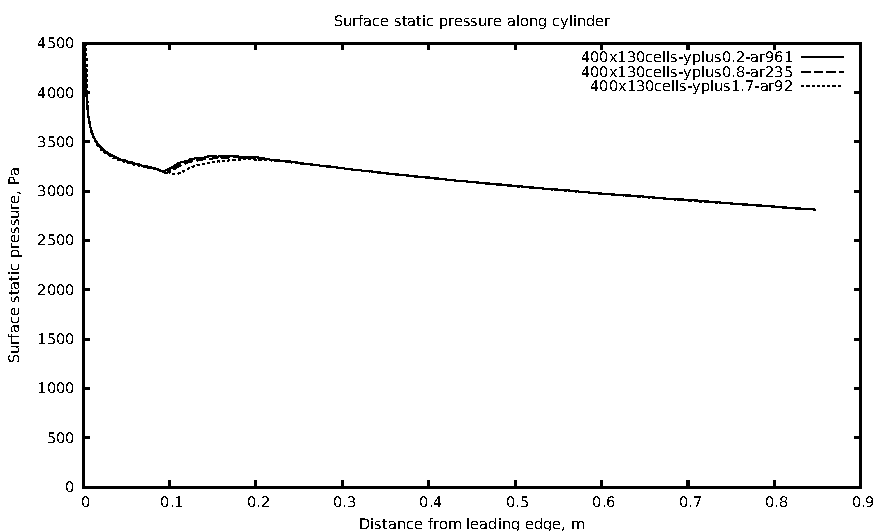
\includegraphics[width=15cm]{./chap3-mallinson-cylinder/figs/compare-yplus-pressure.pdf}
 \end{center}
 \caption{Surface static pressure distribution for grids with different $y^+$ values}
 \label{cylinder-surface-static-pressure-compare-yplus}
%\end{figure}
%\begin{figure}[h]
\vspace{2cm}
 \begin{center}
  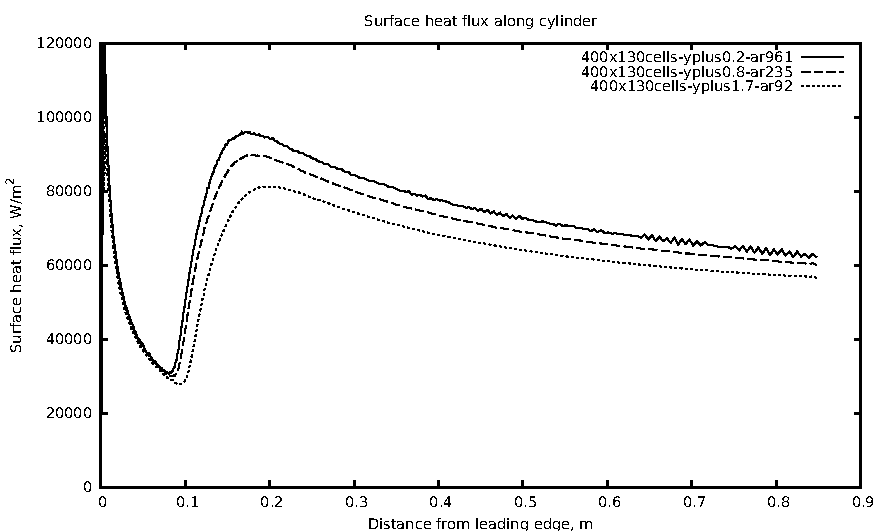
\includegraphics[width=15cm]{./chap3-mallinson-cylinder/figs/compare-yplus-heat-flux.pdf}
 \end{center}
 \caption{Surface heat flux distribution for grids with different $y^+$ values}
 \label{cylinder-surface-heat-flux-compare-yplus}
\end{figure}

It can be observed that only the heat flux distribution is truly sensitive to the 
differences in $y^+$; the average values of pressure distribution are similar for 
all three grids. To quantify the $k$-$\omega$ model's sensitivity to $y^+$ values, the 
$y^+$ value is plotted against the wall heat flux value at an arbitrary location 
($x$ = 0.8\,m) for each grid in Figure~\ref{cylinder-surface-heat-flux-compare-yplus},
and shown in Figure~\ref{cylinder-compare-surface-heat-flux-for-different-yplus}. 
A line fitted through these points is extrapolated to estimate the wall heat flux value 
if an infinitesimally small $y^+$ is used. A comparison between this extrapolated 
wall heat flux value to that for $y^+$ = 0.2 gives a difference of approximately 
1\%. For a $y^+$ of 0.8, the difference is about 6\% and for a $y^+$ of 1.7, this
difference is about 13\%. For this test case, where the experimental uncertainties 
are about $\pm$5\%, the use of the numerical results from grids with  a $y^+$ 
lesser than 0.8 is acceptable.
%
\begin{figure}[h]
 \begin{center}
  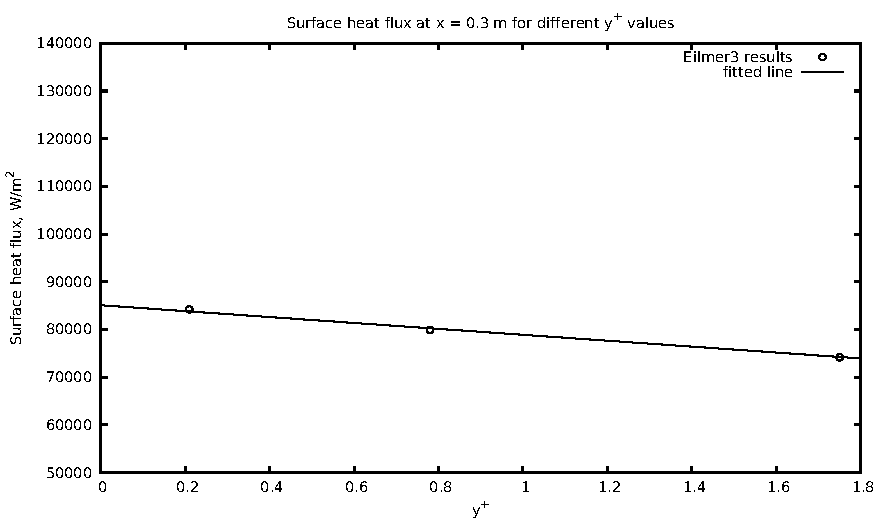
\includegraphics[width=15cm]{./chap3-mallinson-cylinder/figs/yplus-sensitivity.pdf}
 \end{center}
 \caption{Surface heat flux values at $x$ = 0.8\,m for different $y^+$ values}
 \label{cylinder-compare-surface-heat-flux-for-different-yplus}
\vspace{2cm}
\end{figure}

It can also be noted in Figure~\ref{cylinder-surface-heat-flux-compare-yplus} that 
the surface heat flux distribution for the ``400x130cells-yplus0.2-ar961" grid 
become unstable downstream of $x$ = 0.3\,m. This instability is brought about by 
the aspect ratio of the cells. Clustering to the surface to achieve low
$y^+$ values tends to lead to cells with high aspect ratios. To quantify the
effects of cell aspect ratio on the simulations, results from grids with different
cell aspect ratios are plotted in Figure~\ref{cylinder-surface-heat-flux-compare-aspect-ratio}.
The grids with a maximum cell aspect ratio of around 200 seem stable. When the 
maximum cell aspect ratio is around 577, small instabilities start appearing. For
grids with maximum cell aspect ratio higher than 600, significant instabilities
can be seen in the surface heat flux traces. It is therefore recommended that
maximum cell aspect ratios be kept below 600 for all simulations. Since this
recommendation is deduced from a test case which has a relatively simple flow,
it is highly possible that a smaller aspect ratio is needed in regions with 
stronger flow gradients or flow separation.
%
\begin{figure}[h]
 \begin{center}
  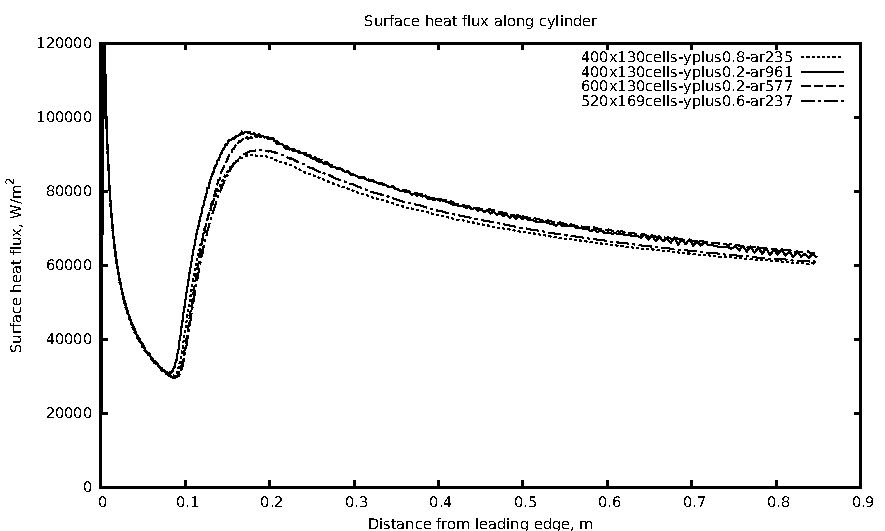
\includegraphics[width=15cm]{./chap3-mallinson-cylinder/figs/compare-aspect-ratio-heat-flux.pdf}
 \end{center}
 \caption{Surface heat flux distribution for grids with different maximum cell aspect ratio}
 \label{cylinder-surface-heat-flux-compare-aspect-ratio}
\end{figure}

Among the nine grids listed in Table~\ref{table-cylinder-grids}, the 
``600x130cells-yplus0.2-ar577" grid is taken to be the most suitable
one for comparison with the experimental data - it is sufficiently 
grid-converged for both boundary layer profiles and surface pressure 
and heat flux distributions, it has a maximum aspect ratio of less
than 600, and it has an average $y^+$ of about 0.2. The numerical results
for this grid are plotted against the experimental data in 
Figures~\ref{cylinder-surface-static-pressure} and \ref{cylinder-surface-heat-flux}.
The computed surface static pressures agree well with those measured experimentally. 
The slight dip in the surface static pressure distribution at $x$ $\approx$ 0.1\,m 
in Figure~\ref{cylinder-surface-static-pressure} is an artefact of the 
turbulence model transitioning the boundary layer from a laminar to a turbulent 
state. 

The surface heat flux distribution in Figure~\ref{cylinder-surface-heat-flux}
can be divided into three regions - laminar region between $x$ $\approx$ 0.0\,m 
and 0.1\,m, transitioning region between $x$ $\approx$ 0.1\,m and 0.16\,m, and
turbulent region from $x$ $\approx$ 0.16\,m onwards. The laminar surface heat 
flux distribution is well predicted by Eilmer3. The transitioning region also
appears to be well modelled by the $k$-$\omega$ model in Eilmer3. An interesting 
point to note here is that even though the only variable fixed by the user in 
this simulation is the transitioning location, the overall transitioning process 
(the peak, slope and length of surface heat flux distribution in the transitioning 
region) is predicted quite well by the $k$-$\omega$ model. For the turbulent
region, the simulated surface heat flux distribution from $x$ $\approx$ 0.16\,m to
$x$ $\approx$ 0.5\,m matches the experimental data. However, the numerically 
predicted heat flux deviates progressively from the experimental values downstream 
of $x$ $\approx$ 0.5\,m.
%
\begin{figure}[h]
 \begin{center}
  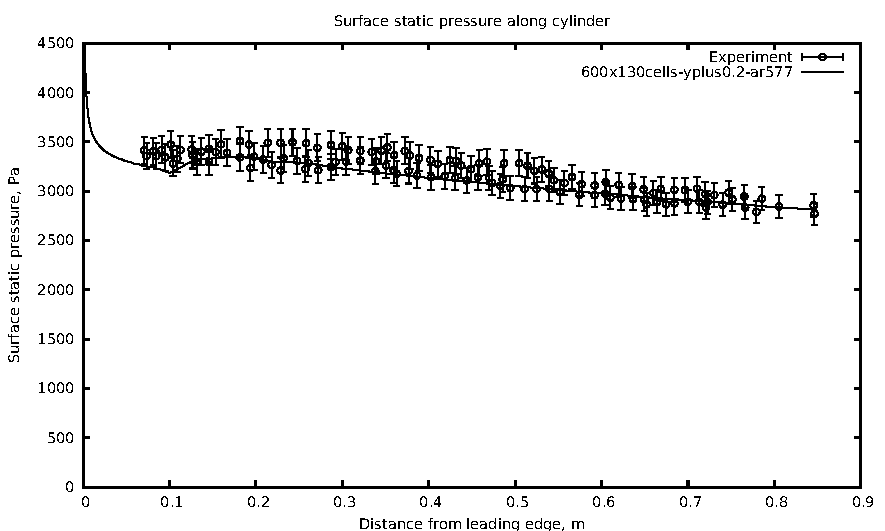
\includegraphics[width=15cm]{./chap3-mallinson-cylinder/figs/final-pressure.pdf}
 \end{center}
 \caption{Surface static pressure distribution}
 \label{cylinder-surface-static-pressure}
%\end{figure}
%\begin{figure}[h]
\vspace{2cm}
 \begin{center}
  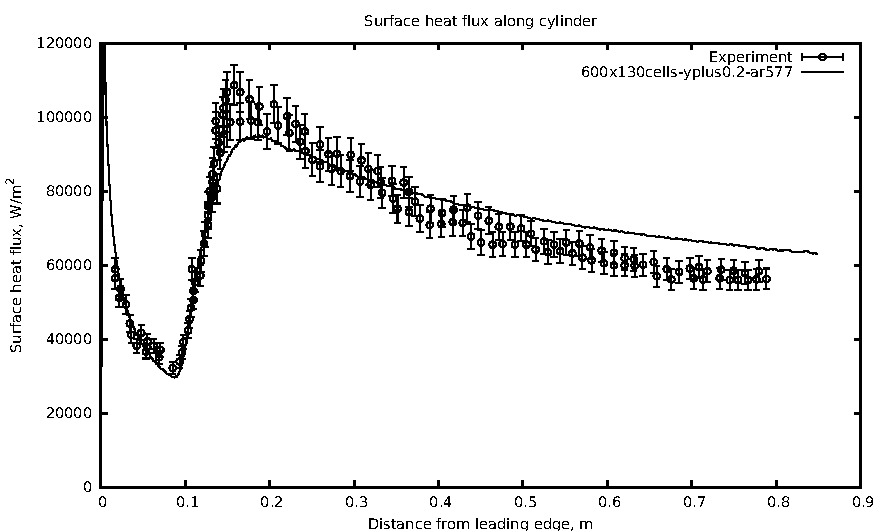
\includegraphics[width=15cm]{./chap3-mallinson-cylinder/figs/final-heat-flux.pdf}
 \end{center}
 \caption{Surface heat flux distribution}
 \label{cylinder-surface-heat-flux}
\end{figure}

In summary, this validation exercise shows that Eilmer3 can be used to predict the
development of an axisymmetric flow on a cylinder. It also shows that the simulated
surface heat flux distribution is more sensitive to the geometrical properties of
the first wall cell (distance from cell centre to wall and cell aspect ratio) than 
the surface pressure distribution. In addition, this exercise also demonstrates that
$y^+$ values and maximum cell aspect ratios should be kept below 1 and 600 respectively. 
The validation of this test case can be extended to test the $k$-$\omega$ model's 
capability in predicted shock-induced separation of an axisymmetric boundary layer. 
Experimental data for the shock-induced separation extension to this test case can be 
found in Boyce \& Hillier \cite{Boyce2000}.

\subsection{udf-supersonic-in.lua}
\label{section-udf-supersonic-in-lua}
\topbar
\lstinputlisting[language={}]{./chap3-mallinson-cylinder/udf-supersonic-in.lua}
\bottombar
